\documentclass[../../thesis.tex]{subfiles}

\begin{document}
\TODO{Should i elaborate on anything? Feels a bit brief, but i am kinda stuck}
Our work involves building a framework that leverage non-contrastive self-supervised learning (SSL) to improve representation learning in a Vector Quantized Variational Autoencoder (VQVAE) type model. Additionally, we fit a prior model on the learned representations. This section presents the works related to ours. To the best of our knowledge, enhancing VQ-based tokenization models with SSL methods has not yet been investigated in the time series domain. Therefore, the related works consist of models used as different components in our model.\newline

We base our model on a simplified version of TimeVQVAE, which utilize a bidirectional transformer model, MaskGIT, for prior learning. Although our non-contrastive SSL extension could use any model with a siamese architecture, we experiment with the proven methods Barlow Twins and VIbCReg.

\section{MaskGIT}

The Masked Generative Image Transformer (MaskGIT), introduced in \cite{chang2022maskgit}, is a generative transformer model for image synthesis developed by Google Research. The innovation of MaskGIT lies in its token generation method. Unlike traditional autoregressive generative transformers that treat images as a sequence of tokens, MaskGIT employs a bi-directional transformer for image synthesis. This allows MaskGIT to predict tokens in all directions during training, offering a more natural approach to image modeling. During inference, MaskGIT begins with a blank canvas, predicting the entire image iteratively by conditioning on the most confident pixels from previous predictions.\newline

MaskGIT's architecture relies on a tokenization procedure in its first stage. In the original paper, VQGAN \cite{VQGAN} was used for this purpose, focusing on improving the second stage. Therefore, our discussion will primarily address this aspect of the model.

\subsection{Masked Visual Token Modeling (Prior learning)}

For prior learning, the codebook learned in the tokenization procedure is provided with a masking vector, which is the embedding of the special masking token, denoted by $\M$. The input embedding in the bidirectional transformer is initialized with this expanded codebook. For an image $X$ in the dataset $\mathcal{D}$, let $z = \{z_{k_i}\}_{i=1}^N$ denote the sequence of codewords obtained by passing $X$ through the VQ-Encoder. This sequence can equivalently be described as a sequence of indices $s = \{k_i\}_{i=1}^N$. Prior learning involves masking this sequence and training the bidirectional transformer to predict the masked indices.
\newline

Let $s = \{k_i\}_{i=1}^N$ be the sequence of indices described above, and denote the corresponding binary mask by $M = \{m_i\}_{i=1}^N$. During training, a subset of $s$ is replaced by the masking token $\M$ according to the binary mask $M$. This is done by 

\begin{equation}
    s_\text{Mask} = s\odot (1_N-M) +  M\cdot\M,
\end{equation}

where $\odot$ is the Hadamard product (pointwise multiplication), and $1_N$ is a vector with the same shape as $M$ and $s$.\newline

The sampling procedure, or choice number of tokens to mask, is parameterized by a mask scheduling function $\gamma$. The sampling can be summarized as follows

\begin{itemize}
    \item Sample $r \sim U(0,1]$.
    \item Sample $\lceil \gamma(r)\cdot N \rceil$ indices $I$ uniformly from $\{0,\dots,N-1\}$ without replacement. 
    \item Create $M$ by setting $m_i = 1$ if $i\in I$, and $m_i = 0$ otherwise.
\end{itemize}

A forward computation is illustrated in Figure \ref{fig:MaskGIT}, where the bidirectional transformer predicts the probabilities $p(s_i|s_\text{Mask})$ of each masked token. The training objective is to minimize the negative log likelihood of the masked tokes, conditional on the unmasked
\begin{equation}
    \loss_\text{Mask} = -\E_{s\in \mathcal{D}}\left[\sum_{i \in I} p(s_i|s_\text{Mask} ) \right],
\end{equation}
and $\loss_\text{Mask}$ is computed as the cross entropy between the ground truth one-hot token and the predicted token probabilities. 

\begin{figure}[h]
    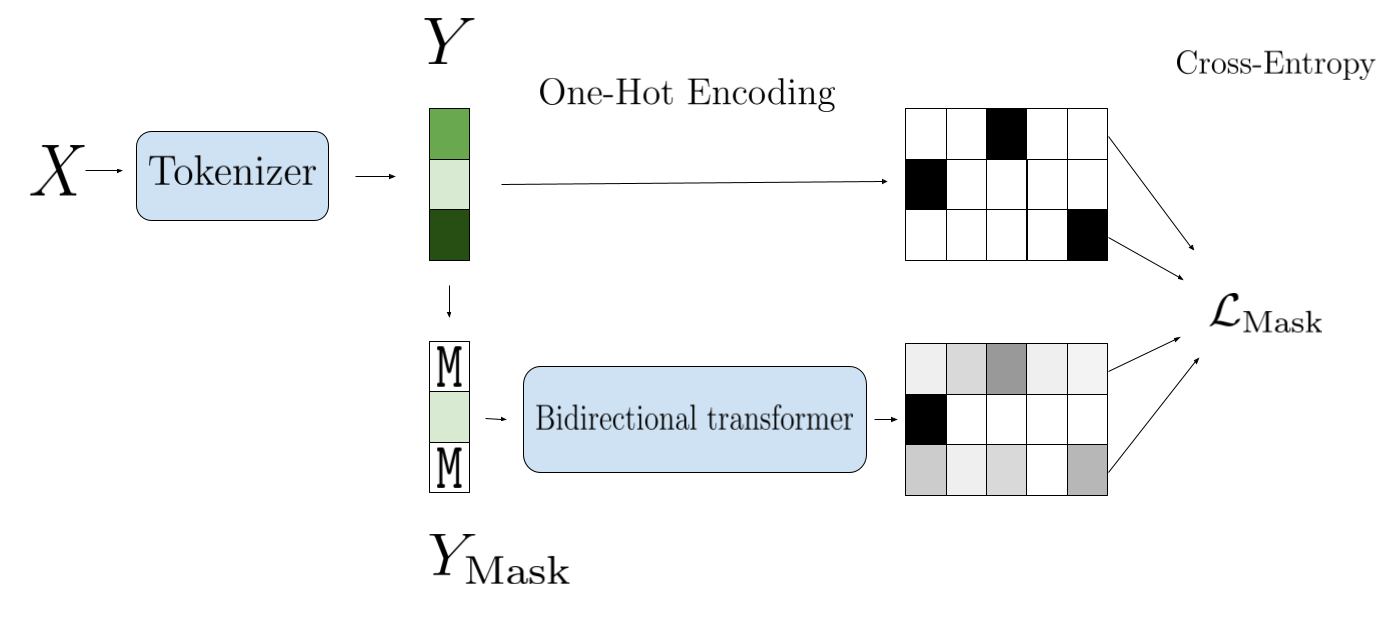
\includegraphics[scale=0.25]{MaskGIT.png}
    \centering 
    \caption{MaskGIT forward computation.}
    \label{fig:MaskGIT}
\end{figure}


\subsection{Iterative Decoding (Sample generation)}

The bi-directional transformer could in principle predict all masked tokens and generate a sample in a single pass by sampling according to the predicted probabilites $p(\widehat{s}_i|s_\text{Mask})$ from a forward pass of an all masked sequence. However, this approach presents certain challenges. To address these, \cite{chang2022maskgit} proposes a novel non-autoregressive decoding method to synthesize samples in a constant number of steps.\newline

The decoding process goes from $t = 0$ to $T$. To generate a sample during inference, the process starts with an all masked sequence, denote as $s_\text{Mask}^{(0)}$. At iteration $t$, the model predicts the probabilities for all the mask tokens, $p(\widehat{s}_i|s_\text{Mask}^{(t)})$, in parallel. At each masked index $i$, a token $s_i^{(t)}$ is sampled according to the predicted distribution, and the corresponding probability $c_i^{(t)}$ is used as a measure of the confidence in the sample. For unmasked tokens, a confidence of $1$ is assigned to the true position.\newline

The number of tokens $s_i^{(t)}$ with highest confidence that are kept for the next iteration is determined by the mask scheduling function. Specifically, $n = \lceil \gamma(t/T)\cdot N \rceil$ of the lower confidence tokens are masked again by calculating $M^{(t+1)}$ as follows

\begin{equation}
    m_i^{(t+1)} = 
    \begin{cases}
        1, \text{ if } c_i < \text{Sort}([c_1^{(t)},\dots,c_N^{(t)}])[n]\\
        0, \text{ otherwise} 
    \end{cases}
\end{equation}

\begin{figure}[h]
    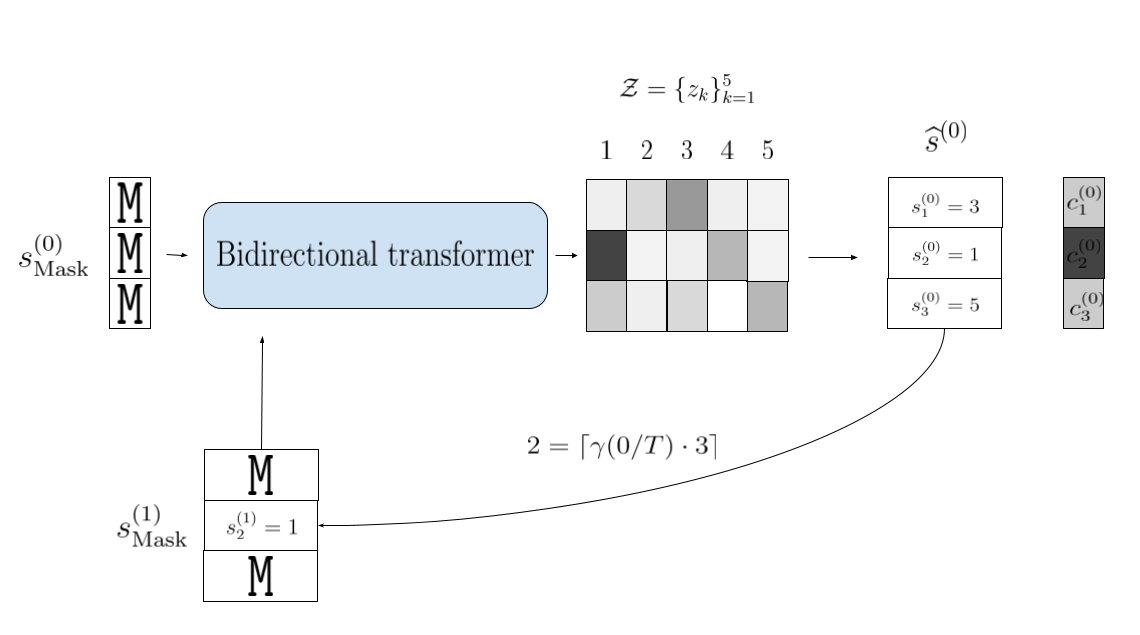
\includegraphics[scale=0.35 ]{Iterative Decoding.png}
    \centering 
    \caption{Illustration of first pass of the iterative decoding algorithm.}
    \label{fig:IterativeDecoding}
\end{figure}

This process is illustrated in Figure \ref{fig:IterativeDecoding}, which shows the first pass of the iterative decoding algorithm. The algorithm synthesizes a complete image in $T$ steps. For image generation, the cosine scheduling function proved to be the most effective across all experiments in the original paper.

\section{TimeVQVAE}

TimeVQVAE is a time series generation model based on VQVAE and MaskGIT. It is the first to our and the authors knowledge that utilizes vector quantization (VQ) to address the time series generation problem. TimeVQVAE employs a two-stage approach similar to VQVAE, with a bidirectional transformer, akin to MaskGIT, for prior learning. The authors introduce VQ modeling in the time-frequency domain, separating data into high and low-frequency components to better retain temporal consistencies and generate higher quality samples.\newline

In addition to VQ modeling in the time-frequency domain, TimeVQVAE presents a process for sampling jointly from high and low-frequency latent spaces and enables guided class-conditional sampling. By appending a class token, similar to \cite{dosovitskiy2021image}, the model can generate synthetic samples both conditionally and unconditionally.\newline

Our work extends a variation of the TimeVQVAE model without the high-low frequency split, reducing the prior learning method to MaskGIT with the addition of guided class-conditional sampling. Here, we present the tokenization stage and refer the reader to \cite{VQVAE} for details on the prior model training.

\subsection{Tokenization}
The tokenization stage of TimeVQVAE follows a structure similar to VQVAE, with the key difference being the frequency split. An overview of the model is presented in Figure \ref{fig:TimeVQVAE1}. Initially, a time series is mapped to the time-frequency domain using the Short-time Fourier Transform (STFT). The time-frequency representation is then separated into two branches: one zero-padding the high-frequency (HF) region and the other zero-padding the low-frequency (LF) region. Each branch follows the VQVAE architecture, with separate encoders, decoders and codebooks denoted by $E_\LF$, $E_\HF$, $D_\HF$, $D_\HF$ and $\mathcal{Z}_\LF$, $\mathcal{Z}_\HF$ respectively. The output of the decoders are again zero-padded giving $\widehat{u}_\LF$ and $\widehat{u}_\HF$, which are then mapped back to the time domain using the Inverse Short-time Fourier Transform (ISTFT) to produce the reconstructed HF and LF components, $\widehat{x}_\LF$ and $\widehat{x}_\HF$, of the time series.

\begin{figure}[h]
    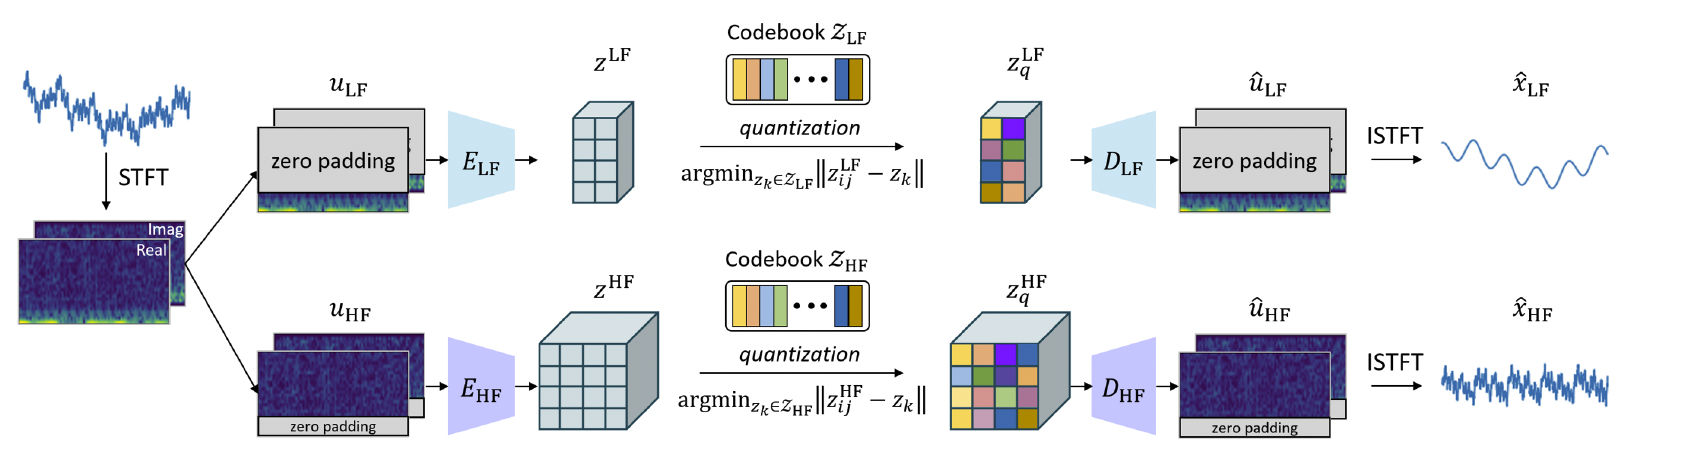
\includegraphics[scale=0.20]{TimeVQVAE1.png}
    \centering 
    \caption{Stage 1: Tokenization. Figure taken with permission from \cite{TimeVQVAE}}
    \label{fig:TimeVQVAE1}
\end{figure}

\subsubsection{Loss}

The codebook loss of TimeVQVAE is similar to the codebook loss presented in Section \ref{section:VQVAE} but reflects the HF-LF split
\begin{equation}
    \label{eq:TimeVQVAE_codebook}
    \begin{aligned}
        \loss_\text{codebook} &= ||\sg[E_{LF}(\Pad_\LF(\STFT(x)))] - z_q^{\LF} ||_2^2 \\
                              &+ ||\sg[E_{HF}(\Pad_\HF(\STFT(x)))] - z_q^{\HF} ||_2^2 \\
                              &+ \beta||E_{LF}(\Pad_\LF(\STFT(x))) - \sg[z_q^{\LF}]||_2^2 \\
                              &+ \beta||E_{HF}(\Pad_\HF(\STFT(x))) - \sg[z_q^{\HF}]||_2^2,
    \end{aligned}
\end{equation}
where $\Pad_{[\cdot]}$ denotes the zero-padding operation. 
The reconstruction loss is computed both on time and time-frequency reconstructions and is given by
\begin{equation}
    \label{eq:TimeVQVAE_recons}
    \begin{aligned}
        \loss_\text{recons} &= ||x_\LF - \widehat{x}_\LF ||_2^2 + ||x_\HF - \widehat{x}_\HF ||_2^2\\
                              &+ ||u_\LF - \widehat{u}_\LF ||_2^2 + ||u_\HF - \widehat{u}_\HF ||_2^2.
    \end{aligned}
\end{equation}
The total loss is given by 
\begin{equation}
    \label{eq:TimeVQVAE_loss}
    \loss_\text{VQ} = \loss_\text{codebook} + \loss_\text{recons}.
\end{equation}

To update the codebooks, TimeVQVAE uses an exponential moving average method as presented in Appendix A.1 of \cite{VQVAE}.


\section{SSL}
Our model leverages self-supervised learning algorithms to learn more expressive latent representations. In this section, we present the relevant SSL algorithms for our work: Barlow Twins and VIbCReg.

% One fundamental difference between Barlow Twins and VIbCReg is that the branches are regularized differently. In Barlow Twins the regularization is applied to the cross correlation matrix of the projected output of the two branches, which in general favours scenarios where the two branches produces similar summary statistics. In VIbCReg the covariance term is applied on each branch separately, which works better in scenarios where the branches are different \cite{bardes2022vicreg}.

\subsection{Barlow Twins}

Barlow Twins is a non-contrastive SSL method that applies the \textit{redundancy-reduction principle} \cite{Barlow_origin} from neuroscientist H. Barlow to a pair of identical networks. The key idea is to encourage representations of similar samples to be alike while reducing redundancy between the components of the vectors.\newline

The model produces two augmented views of each sample and projects their representations onto a feature space such that their cross-correlation is close to the identity matrix. This approach enforces both distortion invariance and decorrelated features in the representations.\newline

\begin{figure}[h]
    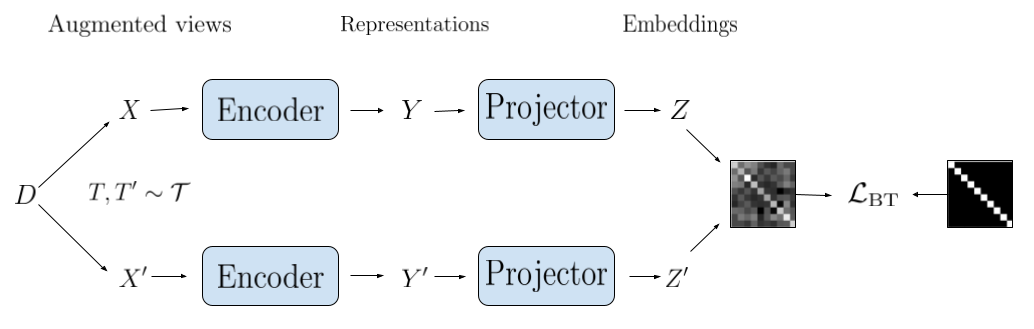
\includegraphics[scale=0.35]{BarlowTwins.png}
    \centering    
    \caption{Overview of the Barlow Twins architecture. Figure inspired by \cite{zbontar2021barlow}}
    \label{fig:BarlowTwins}
\end{figure}

The Barlow Twins algorithm, illustrated in Figure \ref{fig:BarlowTwins}, starts out by creating two augmented views for each datapoint in a batch $D$. These augmentations are sampled from a collection of augmentations $\mathcal{T}$. The batches of augmented views $T(D) = X$ and $T'(D) =X'$, are then passed through an encoder to give representations $Y$ and $Y'$, which are further projected to produce embeddings $Z$ and $Z'$. The embeddings are assumed to be mean centered across the batch dimension. The loss function is calculated using the cross-correlation matrix $\C$ between $Z$ and $Z'$, measuring its deviation from the identity. The Barlow Twins loss is defined as
\begin{equation}
    \label{eq:BTLoss}
    \loss_{\text{BT}} = 
    \overbrace{\sum_i (1 - \C_{ii})^2}^{\text{Invariance}}
    +\lambda  \overbrace{\sum_i\sum_{j\neq i} \C_{ij}^2}^{\text{Redundancy reduction}},
\end{equation}
where
\begin{equation}
    \C_{ij} = \frac{\sum_b z_{b,i}z_{b,j}'}{\sqrt{\sum_b (z_{b,i})^2}\sqrt{\sum_b (z_{b,j}')^2}}.
\end{equation}

The \textit{invariance term} helps make the embeddings invariant to the distortions introduced by the augmentations, pushing the representations closer together. The \textit{redundancy reduction term} decorrelates the different vector components, reducing the information redundancy.\newline

\subsection{VIbCReg}

VIbCReg \cite{lee2024vibcreg} is a non-contrastive SSL model with a siamese architecture based on VICReg \cite{bardes2022vicreg}. It improves upon VICReg by incorporating better covariance regularization and IterNorm \cite{huang2019iterative}. A key difference from Barlow Twins is that variance/covariance regularization is applied to each branch individually.\newline

As with Barlow Twins, a batch $D$ is augmented to create two views and passed through an encoder and projector. The embedding $Z$ and $Z'$ are \textit{whitened} using IterNorm \cite{huang2019iterative}.\newline

\begin{figure}[h]
    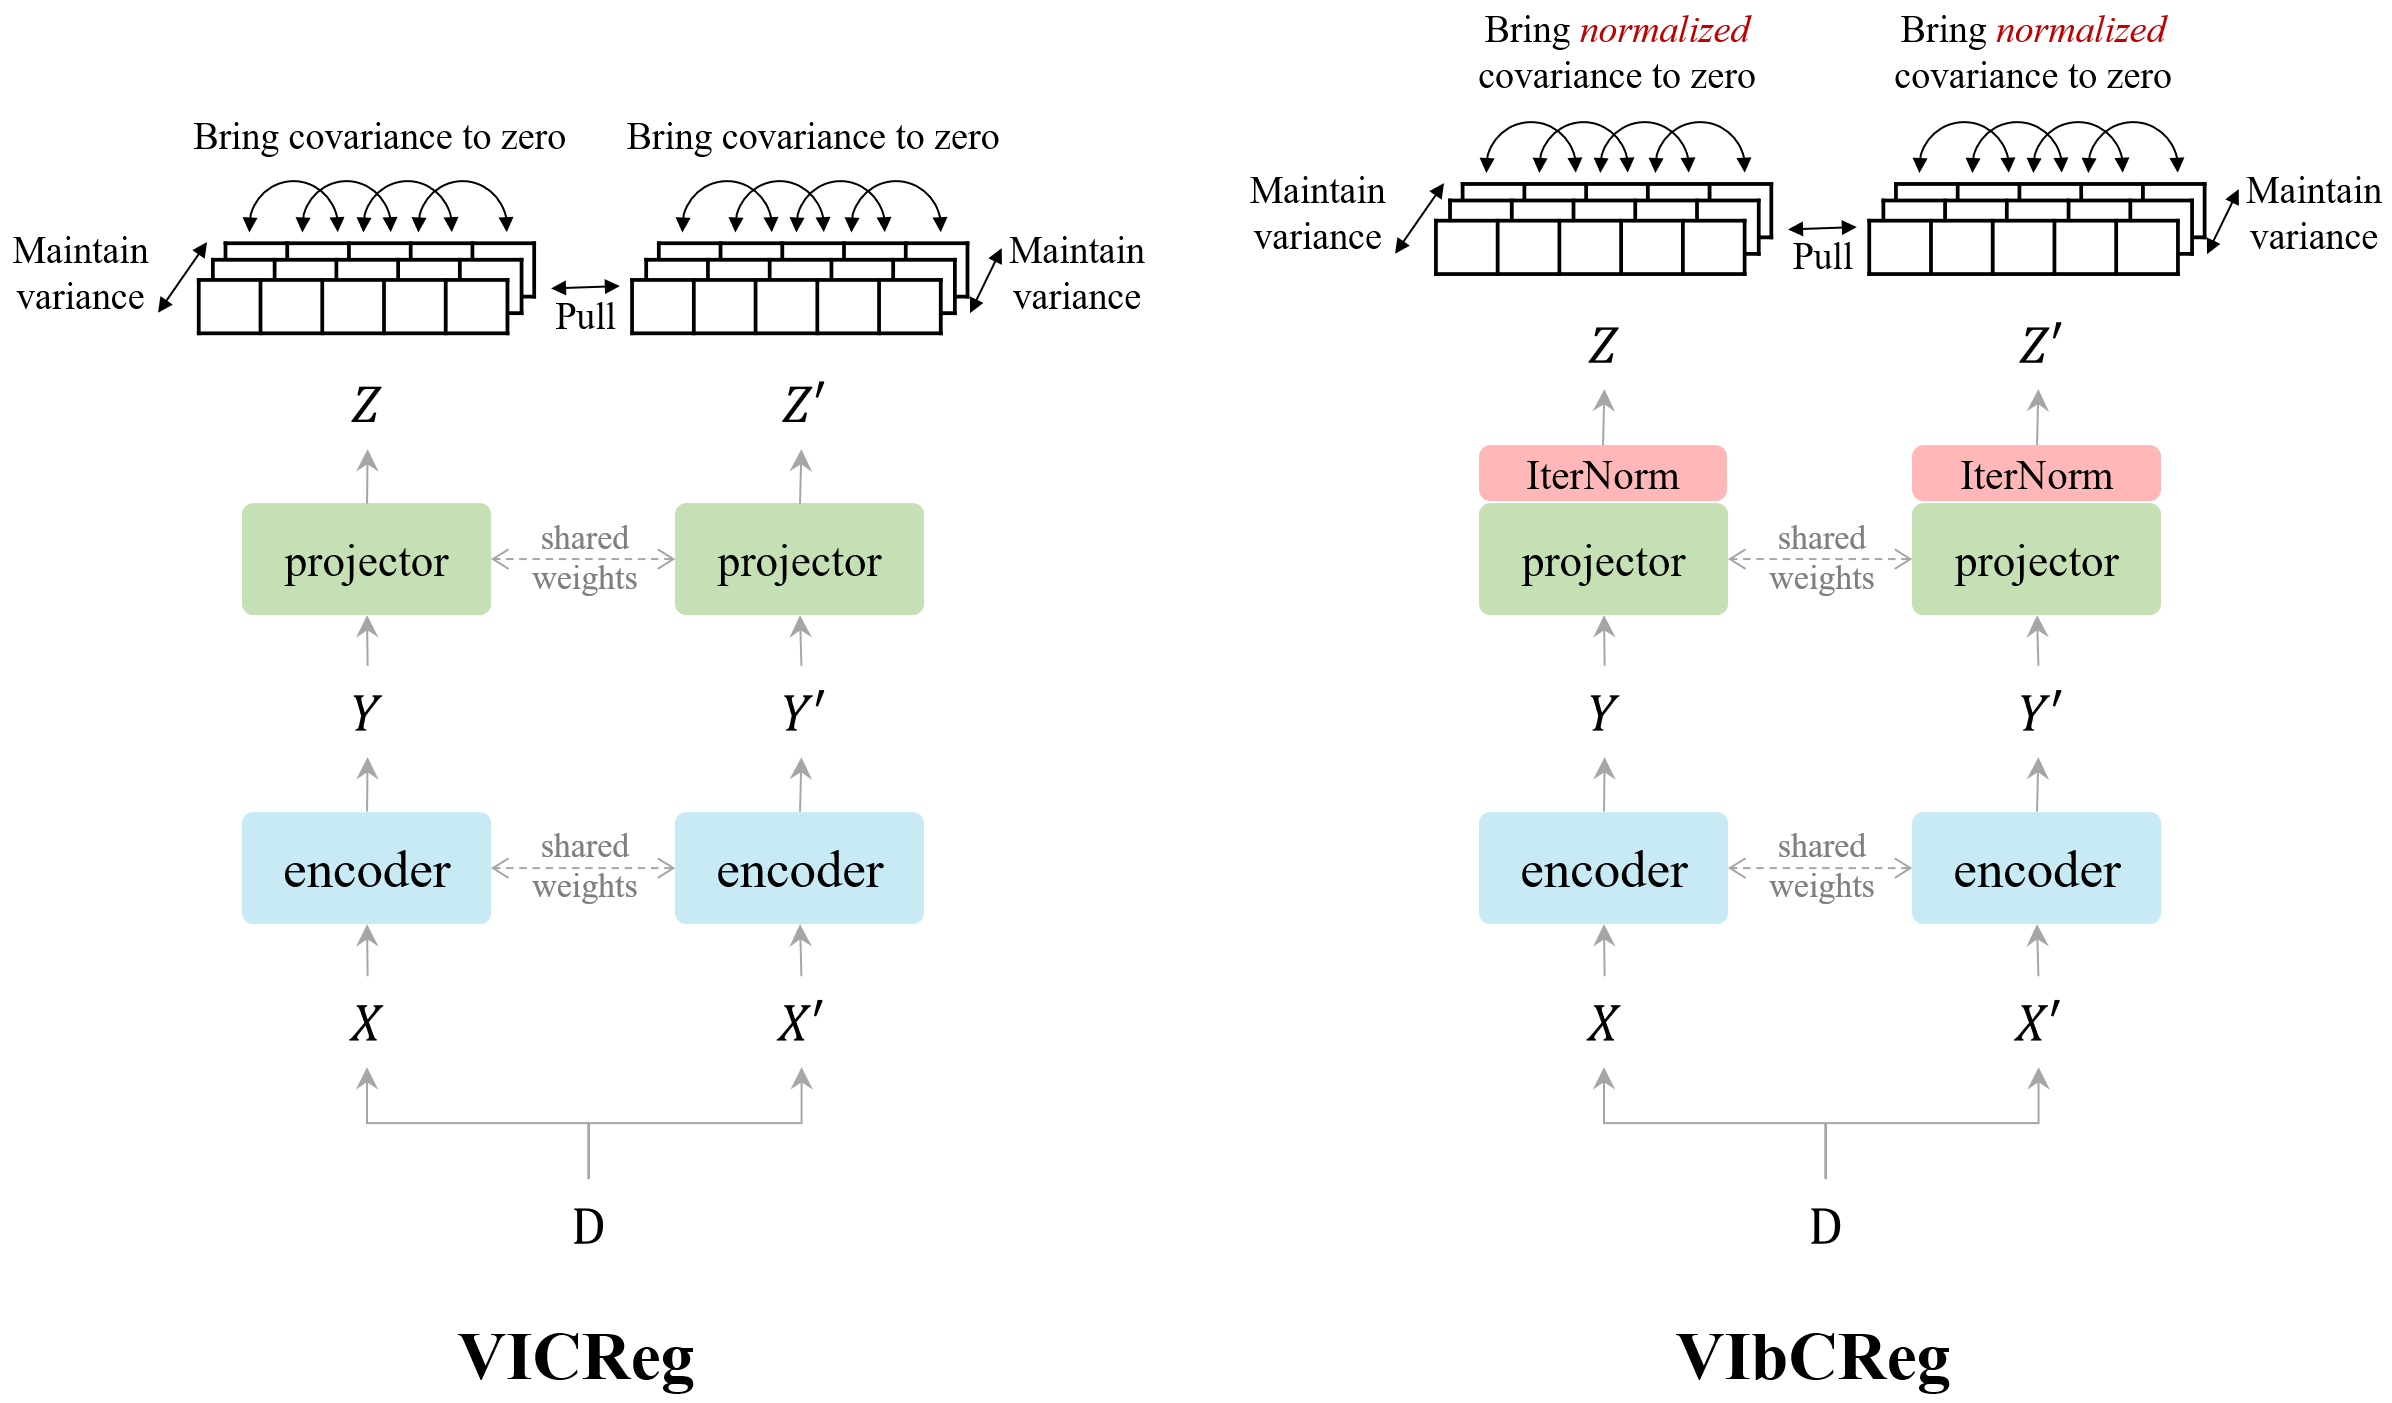
\includegraphics[scale=0.15]{VICReg_VIbCReg.png}
    \centering    
    \caption{Overview of VIbCReg, and comparison with VICReg. Taken with permission from \cite{lee2024computer}}
    \label{fig:VIbCReg}
\end{figure}

The loss consists of a similarity loss between the branches, and feature decoration (FD) loss, and a feature component expressiveness (FcE) term at each branch. Input data is processed in batches, with $Z \in \mathbb{R}^{B\times F}$ where $B$ and $F$ denotes the batch and feature sizes, respectively. We denote a row in $Z$ by $Z_b$ and column by $Z_f$, and similarly for $Z'$.\newline

The similarity loss is defined as the mean square error between the two embeddings
\begin{equation}
    s(Z,Z') = \frac{1}{B} \sum_{b=1}^B || Z_b-Z_b'||_2^2,
\end{equation}
which encourages the embeddings to be similar. The FcE term, which encourages the variation across a batch to stay at a specified level $\gamma$, is defined as 
\begin{equation}
    v(Z) =  \frac{1}{F} \sum_{f=1}^F \max(0,\gamma - \sqrt{\text{Var}(Z_f)+\epsilon}),
\end{equation}
where $\text{Var}()$ is a variance estimator, $\gamma$ is a target value for the standard deviation, which both in VIbCReg and VICReg is set to $1$, and $\epsilon$ is a small scalar to prevent numerical instabilities. 
\newline 

For the FD loss, the embeddings are mean-shifted and normalized along the batch dimension
\begin{equation}
    \widehat{Z}_b = \frac{Z_b-\bar{Z}}{||Z_b-\bar{Z}||_2} \text{ where }  \bar{Z} = \frac{1}{B}\sum_{b=1}^B  Z_b,
\end{equation}
giving 
\begin{equation}
    \widehat{Z} = [\widehat{Z}_1,...,\widehat{Z}_B]^T.
\end{equation}
The normalized covariance matrix is computed as
\begin{equation}
    C(Z) = \frac{1}{B-1}\widehat{Z}^T \widehat{Z},
\end{equation}
before calculating the mean square across all off-diagonal elements to obtain the FD loss
\begin{equation}
    c(Z) = \frac{1}{F^2}\sum_{i\neq j} C(Z)_{ij}^2.
\end{equation}
The total loss is then given by
\begin{equation}
    \label{eq:VIbCRegLoss}
    \loss_\text{VIbCReg} = \lambda s(Z,Z') + \mu [v(Z) + v(Z')] + \nu[c(Z)+c(Z')]
\end{equation}
where $\lambda, \mu$ and $\nu$ are hyperparameters that determine the importance of each term. The normalization of the covariance matrix keep the range of the FD loss small, independent of data, and eases hyperparameter tuning across datasets.

% \begin{equation}
%     C(Z) = \frac{1}{B-1} \left(\frac{Z-\bar{Z}}{||Z-\bar{Z}||_2}\right)^T\left(\frac{Z-\bar{Z}}{||Z-\bar{Z}||_2}\right) \text{ where }  \bar{Z} = \frac{1}{B}\sum_{b=1}^B  Z_b
% \end{equation}


\end{document}